%%%%%%%%%%%%%%
% Fichero: principal.tex
% Autor: Jesús Salido Tercero (https://www.esi.uclm.es/www/jsalido)
% Fecha (creación): febrero 2010 
% Rev. : abril 2025
% Descripción: Plantilla para memoria de TFG 
% (Escuela Sup. de Informática, UCLM). Creada para el curso 
% “LaTeX esencial para preparación de TFG, Tesis y otros documentos 
% académicos” (Esc. Sup. Informática-UCLM)
%
%### Compilación 
%
% Esta plantilla ha sido preparada para compilarse con `pdflatex`  
% (bibliografía con `bibtex`). Se recomienda emplear una distribución
% de LaTeX como MiKTeX o TeXLive.
%
% Una versión revisada de esta plantilla está disponible en Overleaf para
% trabajar online. 
%
% Si deseas acceder a la versión de desarrollo puedes encontrarla en GitHub:
%	https://github.com/JesusSalido/TFG_ESI_UCLM
%%%%%%%%%%%%%%

% Al llamar a la clase puedes pasarle opciones que indican el idioma pral.
% del documento (spanish o english), el tipo de dispositivo (normal, para 
% imprimir en papel y screen para leer en pantalla), y si se desea
% numeración de páginas en el pie (pageonfooter=true) o en la cabecera
% (pageonfooter=false).
\documentclass[final, % final o draft (sin figuras)
				english, % Idioma pral. (spanish o english)
				device=screen, % Tipo de dispositivo (normal o screen)
				pageonfooter=false % Paginación en el pie
]{TFGesi}

% -------------------------
% EDITA: Los datos del documento con la información de tu trabajo.
%
% IMPORTANTE: Todos los campos son obligatorios, 
% pero \cotutline se puede dejar vacío.
%
% Algunos datos deben declararse en el idioma alternativo al pral.
% del documento. Estos datos se emplean en el resumen en el idioma
% alternativo.  
%
% La clase TFGesi los usa para generar el contenido personalizado.
% Puedes usarlos en cualquier parte del documento suprimiendo 
% el carácter '@', p.ej., \titulo
% -------------------------
\makeatletter 
\@titulo{MADTrack: Distributed System for Dataset and Artificial Intelligence Model Management} % 1ª Línea
\@tituloCorto{MADTrack: SD de gestión de conjuntos de datos y modelos de IA} % En idioma pral.
\@tituloCortoAlt{MADTrack: DS for Dataset and AI Model Management} % En idioma alt.
\@autoria{Miguel Ángel Ruiz Arreaza}
\@email{miguelangel.ruiz9@alu.uclm.es}
\@autorline{Author: \autoria}
\@tutline{Tutor: José Luis Espinosa Aranda}
\@cotutline{Co-tutor: Pablo Tomás Toledano González}
%\@cotutline{} % Si no procede dejar vacío (NO BORRAR)
\@instEdu{UNIVERSIDAD DE CASTILLA-LA MANCHA}
\@centroEdu{ESCUELA SUPERIOR DE INFORMÁTICA}
\@titulacion{BACHELOR IN COMPUTING ENGINEERING} % En idioma pral.
\@titulacionAlt{GRADO EN INGENIERÍA INFORMÁTICA} % En idioma alt.
\@especialidad{Coursed intensification: Computer Engineering} 
\@depto{Tutor's Department: }
\@tipoDoc{BACHELOR DISSERTATION} % En idioma pral.
\@tipoDocAlt{TRABAJO FIN DE GRADO} % En idioma alt.
\@mesTF{Julio}        	% Mes de defensa
\@monthTF{July}        	% En inglés
\@yearTF{2025}        	% Año de defensa
\@cityTF{Ciudad Real}	% Ciudad de defensa
\@escudo{esiLogo}       % Logo centro (pdf, png o jpg)
\makeatother 
% -------------------------

% Palabras clave: Son importantes para facilitar búsqueda en Internet
% Se añaden como metadatos al PDF final.
\setkeywords{% (hasta 5 o 6 máx.)
	Escuela Superior de Informática, %
	UCLM, %
	TFG, %
	\LaTeX, %
	\TeX Live, %
	AI, %
	Deep Learning, %
	Distributed System, %
	Dataset, %
	configuration management %
} 

% -------------------------
% CARGAR GLOSARIO
% -------------------------
\makeglossaries

% -------------------------
% CUERPO del documento
% -------------------------
% Para pruebas, limita los ficheros incluidos.
%\includeonly{} 
\begin{document}

% -------------------------
% ACRÓNIMOS
% -------------------------

\newacronym{AI}{AI}{Artificial Intelligence}
\newacronym{CV}{CV}{Computer Vision}
\newacronym{PaaS}{PaaS}{Platform as a Service}
\newacronym{CSV}{CSV}{Comma Separated Values}
\newacronym{JSON}{JSON}{JavaScript Object Notation}
\newacronym{ML}{ML}{Machine Learning}

% -------------------------
% Portadas, créditos, resumen, agradecimiento, notación e índices. 
\frontmatter
%\input{./Anexos/PortadaETSII} % Por ej.,: Otras portadas
%\includepdf{fichero_portada.pdf} % Incluso como fichero PDF

% -------------------------------------------------------------------------
% PORTADA PRAL. (1)
% -------------------------------------------------------------------------

% \portadaOld % Portada pral.
\portadaNew

% -------------------------------------------------------------------------
% PORTADA INTERIOR (2)
% -------------------------------------------------------------------------
\portadaInt %Portada interior


% -------------------------
% CRÉDITOS
% -------------------------
\begin{creditos}[\titulo] % Editar a conveniencia (se pasa el título deseado)
The author may choose the license type they wish. This document is distributed under license CC BY-NC-SA 4.0. The full text of the license is available at \url{https://creativecommons.org/licenses/by-nc-sa/4.0/}. The copy and distribution of this work is permitted in all parts of the world, without royalties and in any medium, as long as this notice is preserved. In addition, permission is granted to copy and distribute translations of this book from the English original to another language, provided that the copyright notice and this permission notice are preserved in all copies.

\noindent \includegraphics[width=0.15\linewidth]{by-nc-sa}

% Para citar este plantilla empleando bibtex puedes emplear el registro siguiente:
%@www{salidoTFG,
%  author       = {Jesús Salido},
%  title        = {Plantilla guía de TFG para la ESI-UCLM},
%  year         = {2019},
%  editor       = {GitHub},
%  organization = {Universidad de Castilla-La Mancha},
%  url          = {https://github.com/JesusSalido/TFG_ESI_UCLM},
%  doi          = {10.5281/zenodo.4574562}
%}
\end{creditos}


% -------------------------
% CALIFICACIÓN DEL TRIBUNAL  (No necesario en versión electrónica)
% -------------------------
%\tribunal % Página opcional para calificación 


% -------------------------
% DEDICATORIA 
% -------------------------
\begin{dedicatoria} % (no confundir con los agradecimientos)
\emph{To my family, close friends, fellow colleagues, classmates and professors \\ % A alguien muy especial
For their patience and for accompanying me and showing me the way through this exciting journey.}
\end{dedicatoria}

\pagestyle{plain}	% Páginas sólo con numeración inferior al pie


% -------------------------
% RESÚMENES:
% -------------------------

% EDITAR: Resumen en idioma alternativo default=english (máx. 1 pág.)
%---
\begin{resumenAlt}[english]{\tituloCortoAlt} 
% Se pasa el idioma (opcional) y título

\emph{<<What>>}

Artificial Intelligence is on the rise, and many companies are striving to create a wide-ranging variety of models to help themselves and their customers in an equally wide range of specific tasks. This inevitably translates into multiple model trainings being performed a year and, in many cases, many datasets being created or modified in the same time interval. 
Such is the case of UBOTICA Technologies: a Space:AI company that works in Computation \emph{on the edge}, delivering AI solutions integrated in embedded systems incorporated in spatial modules, which come with limited space for storing data and computing power. The development of these solutions requires multiple training and deployment iterations,
which over the years presented challenges in maintaining optimal traceability across their AI training environments, increasing the time required to search for a specific AI training configuration. 


\emph{<<How>>}

MADTrack is a distributed configuration management system with the purpose of putting order to the aforementioned challenges. It will store, track and manage all changes within datasets and AI model configurations. The main 
restrictions over the development of the system are the limited storage space of the company for this resources (the management of the evolution of datasets and models has to be done efficiently), the distributed nature of the environment where the items 
are stored and managed and the need for the system to be integrated in a greater processing workflow. The development of the system will be divided in a series of prototypes with an iterative and incremental approach, following continuous testing policies.



\emph{<<Conclusion>>}

The resulting system will consist of a distributed system following the client-server application, with a local or remote server attending requests from multiple clients sending requests by means of a software wrapper library which in turn will interact with other open-source technologies.

\end{resumenAlt}

% EDITAR: Resumen en idioma pral. default=spanish (máx. 1 pág.) 
\begin{resumenPral}[spanish]{\titulo} % Se pasa el idioma (opcional) y título

\emph{<<Que>>}

La Inteligencia Artificial está en ascenso, y muchas empresas están trabajando en la elaboración de una inmensa variedad de modelos que las ayuden tanto a ellas 
como a sus clientes a realizar una variedad de tareas igualmente amplia. Esto provoca que se realicen muchas entrenamientos de modelos al año y, en muchos casos, 
se creen o modifiquen muchos conjuntos de datos en el mismo intervalo de tiempo. Este es el caso de UBOTICA Tecnologías: una empresa de Space:AI que apuesta por la
computación \emph{on the edge} para ofrecer soluciones de Inteligencia Artificial integradas en sistemas empotrados en módulos espaciales, que tienen un espacio de 
almacenaje y poder computacional limitado. El desarrollo de estas soluciones requiere de varias iteraciones de entrenamiento y despliegue, lo que ha llevado a un desorden
caótico de conjuntos de datos y modelos difícilmente identificables, lo que dificulta la búsqueda de un modelo o configuración de entrenamiento específica. 

\emph{<<Como>>}

MADTrack es un sistema de gestión de configuración distribuido que tiene el propósito de ponerle orden al caos configuracional previamente mencionado. El sistema almacenará, 
rastreará y gestionará todas las modificaciones de conjuntos de datos y configuraciones de modelos IA.Las principales
restricciones que tiene el desarrollo del sistema son el espacio de almacenamiento limitado de la empresa para estos recursos (la evolución de conjuntos de datos y modelos debe ser 
registrada de manera eficiente), la naturaleza distribuida del entorno donde se almacenan y gestionan los elementos y la necesidad de la integración del sistema en un gran flujo de
procesamiento. El desarrollo del sistema se dividirá en una serie de prototipos con un enfoque iterativo y incremental, siguiendo políticas de pruebas continuas.


\emph{<<Conclusiones>>}

El sistema resultante consistirá en un sistema distribuido que sigue la arquitectura cliente-servidor, con un servidor local o remoto atendiendo las solicitudes de varios clientes enviando 
solicitudes a través de una biblioteca Software del tipo Wrapper que a su vez se interactúe con otras tecnologías de software abiertas. 

\end{resumenPral}




% Ajuste al idioma pral.
\ifbool{ESI@spanish}{\selectlanguage{english}}{\selectlanguage{spanish}}


% -------------------------
% AGRADECIMIENTOS (máx. recomendable: 1 pág.)
% -------------------------
\auxchapter{Agradecimientos} % Editar a conveniencia
Aunque es un apartado opcional, haremos bueno el refrán \emph{<<es de bien nacidos, ser agradecidos>>} si empleamos este espacio como un medio para agradecer a todos los que, de un modo u otro, han hecho posible que el trabajo realizado \emph{llegue a buen puerto}. Esta sección es ideal para agradecer a directores, profesores, mentores, familiares, compañeros, amigos, etc. 

Estos agradecimientos pueden ser tan personales como desees e incluir anécdotas y chascarrillos, pero recuerda que \emph{no deberían ocupar más de una página}.

\firma % Nombre, lugar y año (automático, no cambies)


% -------------------------
% -NOTACIÓN: Lista de símbolos con significado especial.
% -------------------------
\auxchapter{Notación y acrónimos}
\section*{Notacion}
(Texto aclaratorio \emph{-suprime-}). Ejemplo de lista con notación (o nomenclatura) empleada en la memoria del TFG. Debes editarla según las necesidades de tu trabajo intenta que sea informativa y evita que incorpore información obvia.\footnote{Se incluye únicamente con propósito de ilustración, ya que el documento no emplea la notación aquí mostrada.}

\begin{tabular}{r r p{0.8\linewidth}}
$A, B, C, D$	& : & Variables lógicas \\
$f, g, h$		& :	& Funciones lógicas \\
$\cdot$			& : & Producto lógico (AND), a menudo se omitirá como en $A 
B$ en lugar de $A \cdot B$\\
$+$				& : & Suma aritmética o lógica (OR) dependiendo del 
contexto\\
$\oplus$		& : & OR exclusivo (XOR)\\
$\overline{A}$ o ${A}'$	& : & Operador NOT o negación
\end{tabular}

\section*{Lista de acrónimos}
% OJO: Esta lista debería estar ordenada alfabeticamente (hacer de modo manual).
(Texto aclaratorio \emph{-suprime-}). Ejemplo de lista \emph{ordenada alfabéticamente} con los acrónimos empleados en el texto. Se pueden omitir aquellos acrónimos que son reconocidos en el contexto académico (p.~ej., PhD), aunque aquí se han incluido a efectos ilustrativos.


% -------------------------
% ÍNDICES: Elimina los innecesarios.
% -------------------------
\idxGral
\idxFiguras
\idxTablas
\idxListados
\idxAlgoritmos
%---


 % Contiene portadas y otros elementos preliminares
% -------------------------

% -------------------------
% Capítulos
\mainmatter
%\onehalfspacing % Ajusta interlineado a 1.5 líneas

% Ubicados en ./Caps por mayor comodidad. 
% Pueden modificarse los nombres y rutas a conveniencia.
% No se precisa nombre precedido por número (se hace por claridad).
\chapter{Introduction}
\label{cap:Introduction}

With the passage of time, the development of \acrfull{AI} has become of increasing interest due to the powerful tools it can provide to any
organisation \cite{AIRise}. Since the development of \emph{The Bombe}, the machine that was able to decode the \emph{Enigma} machine in 1939,
passing through a whole set of ups and downs and even a silent winter before its comeback in 2015 thanks to Deep Learning, Artificial Intelligence
is being applied in a number of fields, sometimes even reaching the point of having the potential of threatening human safety and raising awareness
of the need of regulations for its use.

The development of these models has been made possible thanks to the contribution of a number of organisations, such as Google, Microsoft and OpenAI,
which invested an objectively significant amount of time and money (reaching a total investment of 24.0 billion dollars in 2018 \cite{AIRise}) to develop systems as
broad as the GPT-4 model, which is able to generate text from both imaged and textual inputs \cite{GPT4}, and is capable of helping professionals in solving
doubts in a large number of fields.

With time, the development of these models became increasingly complex and difficult, and this would be reflected in the number of iterations required for
a model to reach the desired level of accuracy in its predictions. Moreover, the application of these techniques on areas where little data was available
made this development even harder. Some companies even started to employ their own resources to gather new data to train their models, which led to a model
having more iterations as the available data grew. Summarizing, a model (and even a dataset) can become complex structures that have many evolutionary
stages within their lifecycle.

Many organisations, aware of the increasing complexity of the lifecycle of datasets and models, saw a market opportunity to develop systems that would manage
these lifecycles in an organized and efficient way, producing the AI and dataset configuration management tools, such as MLFlow \cite{MLflow}, DVC, which were
open source and available to everyone, as well as premium tools such as Neptune.ai, which are \acrfull{PaaS} that provide even further monitoring
capabilities.

The aim of this Final Degree Project is to tackle this issue in a specific particular case. In the coming subsections, the reasons that motivated the elaboration
of this project, along with the challenges it faces and how they will be solved, will be thoroughly described. Finally, an overview of the structure of the document
will be given, so as to give readers the necessary information to follow the development documentation of the project.

\section{Motivation}

It is of common knowledge that Artificial Intelligence has gained significant importance and visibility since the apparition of AlexNet in 2011, which was the basis for Deep Learning along with the possibility
to use GPUs for training neural networks. The development of tools such as the GPT models
have headed a revolution in the way humans solve both simple and complex tasks. A revolution that was made possible with the intervention of multiple
companies and organisations, and a considerable amount of money and time invested in the development of these models \cite{AIRise}.

UBOTICA Technologies is a pioneer company that develops \acrshort{AI} \acrfull{CV} solutions. This means that, as a company, they use Artificial Intelligence
techniques to extract information from images. These solutions are then integrated in embedded systems with limited capabilities, and that are part of a 
bigger, more complex system. The domains where these solutions are used are mainly in the space industry with their new CogniSAT-6 project \cite{UBOTICACS6}, 
and recently even in the culinary industry. The development of the various solutions of the company requires multiple iterations where the models are trained,
validated and tested, either in existing datasets, or in new ones. Moreover, the CogniSAT-6 system has the capability for creating new datasets out of self-taken
images, which may be periodically added to the existing datasets, or even used to replace the existing ones.

This continuous rise of the available models and datasets, paired with a lack of a real control protocol over the new and improved versions of an AI model or dataset,
has often led to situations where an abnormal amount of time is spent searching for the desired dataset, and accessing the necessary training configuration
that produced a specific result.

The aim of MADTrack is to develop a system that establishes a robust configuration management basis for these datasets and \acrshort{AI} models. A system that can integrate
both new and existing datasets and models in a distributed, remote environment, and that will make the best use of the available resources the company dedicates
to this management.

\section{Problems and Solutions}

The main problem to be tackled in this Final Degree Project is the lack of a robust configuration management protocol over the produced datasets and models. Another
problem is the difficulty at not only determining the correct configuration, but also bringing it to the environment where it is going to be used, and the need to adapt the
system to the end users' existing methods to ensure familiarity.

Furthermore, another problem resides within the protocols and deployment requirements of the system, which may need special authentication protocols from
the environment where the system is going to be deployed, as well as from the environment where the models and datasets are stored (which in turn may also differ
from the one where the system is running). All of this may result in the need to develop a distributed system, where many components interact with each other
to satisfy a complex need. Moreover, the system must be easy to integrate in bigger workflows, so the study of the available pipelines the company uses and the 
possible integration points of the system within them may be taken as another problem.

Finally, the last problem is the limitations of the company to dedicate resources for the storage of all the data produced by the model and dataset lifecycles.
The developed system must, hence, make an efficient use of the resources available, so as to maximize the amount of data that could be stored and managed. Also,
the system must be able to adapt to the needs of a growing company, where many requests may be taken concurrently.

For the resolution of all these three problems, the system will be formed by a server that will satisfy requests and perform the necessary storage and
fetching operations to bring both the datasets and the models to the users, whilst the client will be a library that enables the integration of the
necessary items into the configuration management, sending the evolutionary changes of a dataset or model to the server that stores them.


%\begin{table}[H]%
%	\centering
%	\caption{Usos ilícitos de la IA en el TFG}
%	\label{tab:ia}
%	\begin{tabular}{ | p{0.3\linewidth} | p{0.3\linewidth} | p{0.3\linewidth} |}
%		\hline
%		\textbf{Uso de la IA} & \textbf{Descripción} & \textbf{Riesgo} \\
%		\hline
%		Generación completa o parcial de textos para la memoria.&
%		Presentar como propio un texto obtenido casi en su totalidad por una IA. &
%		\textbf{Plagio académico}: el autor no es quien firma el texto.\\
%		\hline
%		Evitar el trabajo intelectual o de análisis. &
%		Usar IA para hacer razonamientos, interpretaciones o críticas sin comprensión real. &
%		Viola los principios de \textbf{evaluación auténtica} y aprendizaje significativo. \\
%		\hline
%		Falsificación de datos. & Generar datos simulados o inexistentes para experimentos, encuestas o estadísticas. &
%		Constituye \textbf{fraude académico}.\\
%		\hline
%		Traducción automática sin revisión. &
%		Entregar traducciones automáticas sin control de calidad. &
%		Puede derivar en \textbf{errores conceptuales}.\\
%		\hline
%	\end{tabular}
%\end{table}


\section{Document Structure}

According to the steps necessary to fully describe the elaboration process of this Final Degree Project, the following structure has been decided:

\begin{enumerate}

\item \textbf{Introduction}. The domain and main problematics are described, as well as what solutions the project will establish to these problematics.

\item \textbf{Objective}. The main objective, as well as the specific objectives of the project, are enumerated and detailed.

\item \textbf{State-of-the-art research}. This chapter contains the results of an extensive research and study of all the concepts and technologies relevant to the development of the project.

\item \textbf{Methodology}. Description of the development framework and methodology to be used, its specific application to the development of the project and the equipment used during it.

\item \textbf{General Configuration Management in MADTrack}. Development chapter focused on specific features of the project, particularly those in relation to General Configuration Management.
\item \textbf{Dataset Configuration Management in MADTrack}. Development chapter focused on specific features of the project, particularly those in relation to Dataset Configuration Management.
\item \textbf{Model Configuration Management in MADTrack}. Development chapter focused on specific features of the project, particularly those in relation to Model Configuration Management.
\item \textbf{MADTrack Tracking Server deployment}. Development chapter that plans the deployment of a specific component of the distributed system, and how does it integrate itself with the rest of the features.

\item \textbf{Results and tests}. Documents how the system was able to be integrated in a real workflow, the steps followed and the results obtained.

\item \textbf{Conclusions}. A summary of the achieved results will be made, as well as the proposal of the future work to be carried out on this project.

\item \textbf{Bibliography}. References to the works that have been used in the elaboration of this document.

\item \textbf{Appendix}. Sections with the auxiliary contents to better understand the project.
\end{enumerate}










\chapter{Objective}
\label{cap:Objective}

The main aim of this chapter is to define the main objective of the project, and also enumerate and detail the specific objectives that will be necessary to fulfill so as to
achieve it. The definition of objectives serves the pupose of providing a better explanation of the work that will be carried out
within the scope of the project, and to provide an indicator of its good progress.

\section{Main Objective}

The main aim of the project is to produce a system capable of tracking the configuration of datasets and \acrshort{AI} models, and is easy to integrate in the internal workflows
and pipelines of the end user (UBOTICA Technologies). The system will also be characterized by its distributed nature, its scalability (it will
make efficient use of the resources, so that an increase on the resources or number of users will make a minimal impact on the system's performance), security (the system must
be prepared for possible attacks, specially from injection and buffer overflow attacks) and robustness (Upon the case of minor failures, the system must remain operational and provide
adequate, meaningful logging).

The system will provide user-friendly mechanisms for accessing the dataset and model configuration database, so the users can make operations on this configuration directly from
their codespaces.

\section{Specific Objectives}

The aforementioned main objective can be divided into a set of partial objectives, also referred to as subobjectives. This final project can be divided into -- subobjectives
that will mark the development progress of the project, which could be in turn considered as finished when all of the subobjectives have been completed, and the resulting system
satisfies the specifications of the main objective.

\begin{itemize}
	\item \emph{Development and deployment planning of a server able to track the configuration of \acrshort{AI} models and datasets.}
	
	A planning will be made regarding the deployment details and the necessary infrastructure to be able to host the Tracking server that will satisfy the requests from the
	other components of the system. These details involve the necessary hardware requirements (Memory, CPU cores, network configuration, available ports ) and 
	software requirements (dependencies and entrypoint scripts) that will be used to design and develop the tracking server, which will be deployed in the future inside of the
	company's intranet infrastructure. It is also necessary to specify how this server will interact with the rest of components of the system and when should it be 
	deployed so as to ensure its proper functioning.

	\item \emph{Development of a library module that manages the configuration management of datasets. Registering changes on their contents.}
	
	Aside from the tracking server, multiple library components will be necessary to manage the configuration of datasets and models. Some of these components will be developed
	under a module that will handle issues regarding the configuration management of datasets. These components will focus on providing code mechanisms that enable the integration
	of new datasets into the system, as well as providing the necessary means to bring the datasets in a specific evolutionary stage to the users.

	\item \emph{Development of a library module that manages the configuration management of AI models, and facilitates the search of models according to their performance.}
	
	Other components of the library will be gathered within a module focused on managing the configuration of Artificial Intelligence models. These components will interact
	with the tracking server in order to track the parameters and metrics produced by the experimental runs of the models performed by the company, and register the final models
	and any other file meaningful to these inside a database.
\end{itemize}
\chapter{State of the art}\label{cap:StateOfTheArt}

This chapter aims to put into context the different concepts and technologies relevant to the development of the project. The following subsections provide an overview of
these technologies, as well as the related concepts they handle, so as to contextualize the upcoming work. In the coming sections, concepts about Artificial Intelligence 
models, datasets and configuration management will be presented. Then, a thorough overview of the available technologies on the market to solve the problems described 
within Chapter 2 will be given.

\section{Datasets}

In a statistical context, and according to a recent article by IBM employees \cite{DatasetIBM}, datasets are collections of organized data. The organization structure comes in
a wide-ranging variety of formats, being the most common ones \acrfull{CSV} and \acrfull{JSON}. The data contained within them can be collected from a number of sources, e.g.
customer interactions, data obtained from distributed IoT devices (In the case of the end users, the satellites equipped with camera devices for taking pictures), or even
public social media.

These arrangements of data are of great value for statistical data analysis, as well as for \acrfull{ML} and other \acrshort{AI} techniques, which require large amounts of
accessible and reliable data to achieve a satisfactory performance. The quality of the data contained within a dataset, according to the definition standard stablished by the
DEEL Workgroup in 2020 \cite{DDS}, is achieved by in turn achieving high ratings in several indicators, such as representativeness, traceability, accuracy, reliability and
consistency, among many other.

With reference to how these datasets are used in \acrlong{AI}, these datasets are usually partially or fully labelled into one out of three categories \cite{DDS}:

\begin{enumerate}

    \item \textbf{Training datasets:} these parts of a dataset (or multiple datasets) will be used during the execution of the model's training algorithm. During the algorithm,
    the model's parameters are automatically adjusted iteratively until the former's convergence.

    \item \textbf{Validation datasets:} Just like the training ones, these are the parts of a dataset(s) used to determine the generalization capability of the trained model To
    a dataset different than the one used in training. As a result, the data scientists will receive information about how the training hyperparameters should be adjusted.

    \item \textbf{Testing datasets:} the data arranged under this category serves the purpose of serving as the test bed where the model's performance will be evaluated. This
    performance is most of the times operational, and the output of the testing phase are the model's performance metrics.

\end{enumerate}

\section{Artificial Intelligence Models}

An \acrlong{AI} model can be considered as a mathematical model which is capable of adjusting its parameters automatically and intelligently in order to reach a goal. This adjustment
may be done based on the outcome previous iterations, also called \emph{experience}. This learning may be assessed by agents external to the model (supervised learning) or may just depend
on the model itself (unsupervised learning). There are cases in which the model assesses itself (reinforcement learning) \cite{introml}.

There are several concepts that are of interest to this project that revolve around this concept of \acrshort{AI} model, as their configuration will highly depend on this:

\begin{itemize}
    \item \textbf{Parameters:} These are the terms of the described mathematical model. They are characterized by their mutability and the lack of external control of their adjustment
    during the training process. They are considered as the \emph{black-box} elements inside a model.

    \item \textbf{Hyperparameters:} These are terms that express qualities on how the model will work. They are characteristically fixed and adjusted by data scientists prior to the 
    training process.

    \item \textbf{Metrics:} Once a model has been trained and validated, the next step is to carry out an evaluation process using the testing datasets. After this evaluation,
    metrics are obtained. They are the main performance indicator for a model, since they explain how the model behaves on average for most of the datasets.

\end{itemize}

\section{Configuration Management}

\begin{quote}
    \emph{"Configuration management is the discipline consisting in the unique identification, controlled storage, change control, and status reporting
            of selected intermediate work products, product components, and products during the life of a system."}
\end{quote}

This definition by the \emph{"Configuration management principles and practice"} book by Anne M. J. Hass \cite{confmanagement} clearly establishes the important features of this discipline. The point
of configuration management is to provide a traceable and accountable control protocol for any kind of system. In this case, our goal is to provide a way to uniquely identify and
control the storage location of models and datasets, in order for the end users to spend less time searching for a particular dataset or a model with very specific parameter,
hyperparameter or metric values.

Some of the ways this can be achieved are the use of version control systems, which allow users to establish different versions for a specific item; status checkers, which track
the different states the item can be found in, or locator systems, which are able to determine the location of the item (specially useful in distributed environments, where the
locations of the items may be physically separated by a considerable distance).

\section{Available technologies and tools for AI model and dataset configuration management}\label{sec:toolAnalysis}

Now that the main concepts relevant to the project have been introduced, it is time to navigate the different solutions that are already available in the market which are capable of
providing the mechanisms for AI model and dataset configuration management.

\subsection{Git LFS}

Git Large File Storage (LFS) is an open-source Git command line extension that enables users to manage and version large files in Git repositories by the means of a Git LFS 
server.

\subsubsection{How does Git LFS work?}

Git LFS reduces the overhead produced at uploading big files as blobs to a repository by storing the real contents of the files in a separate Git LFS server, while storing a 
special pointer file in the repository.


\begin{figure}[H]
    \centering
    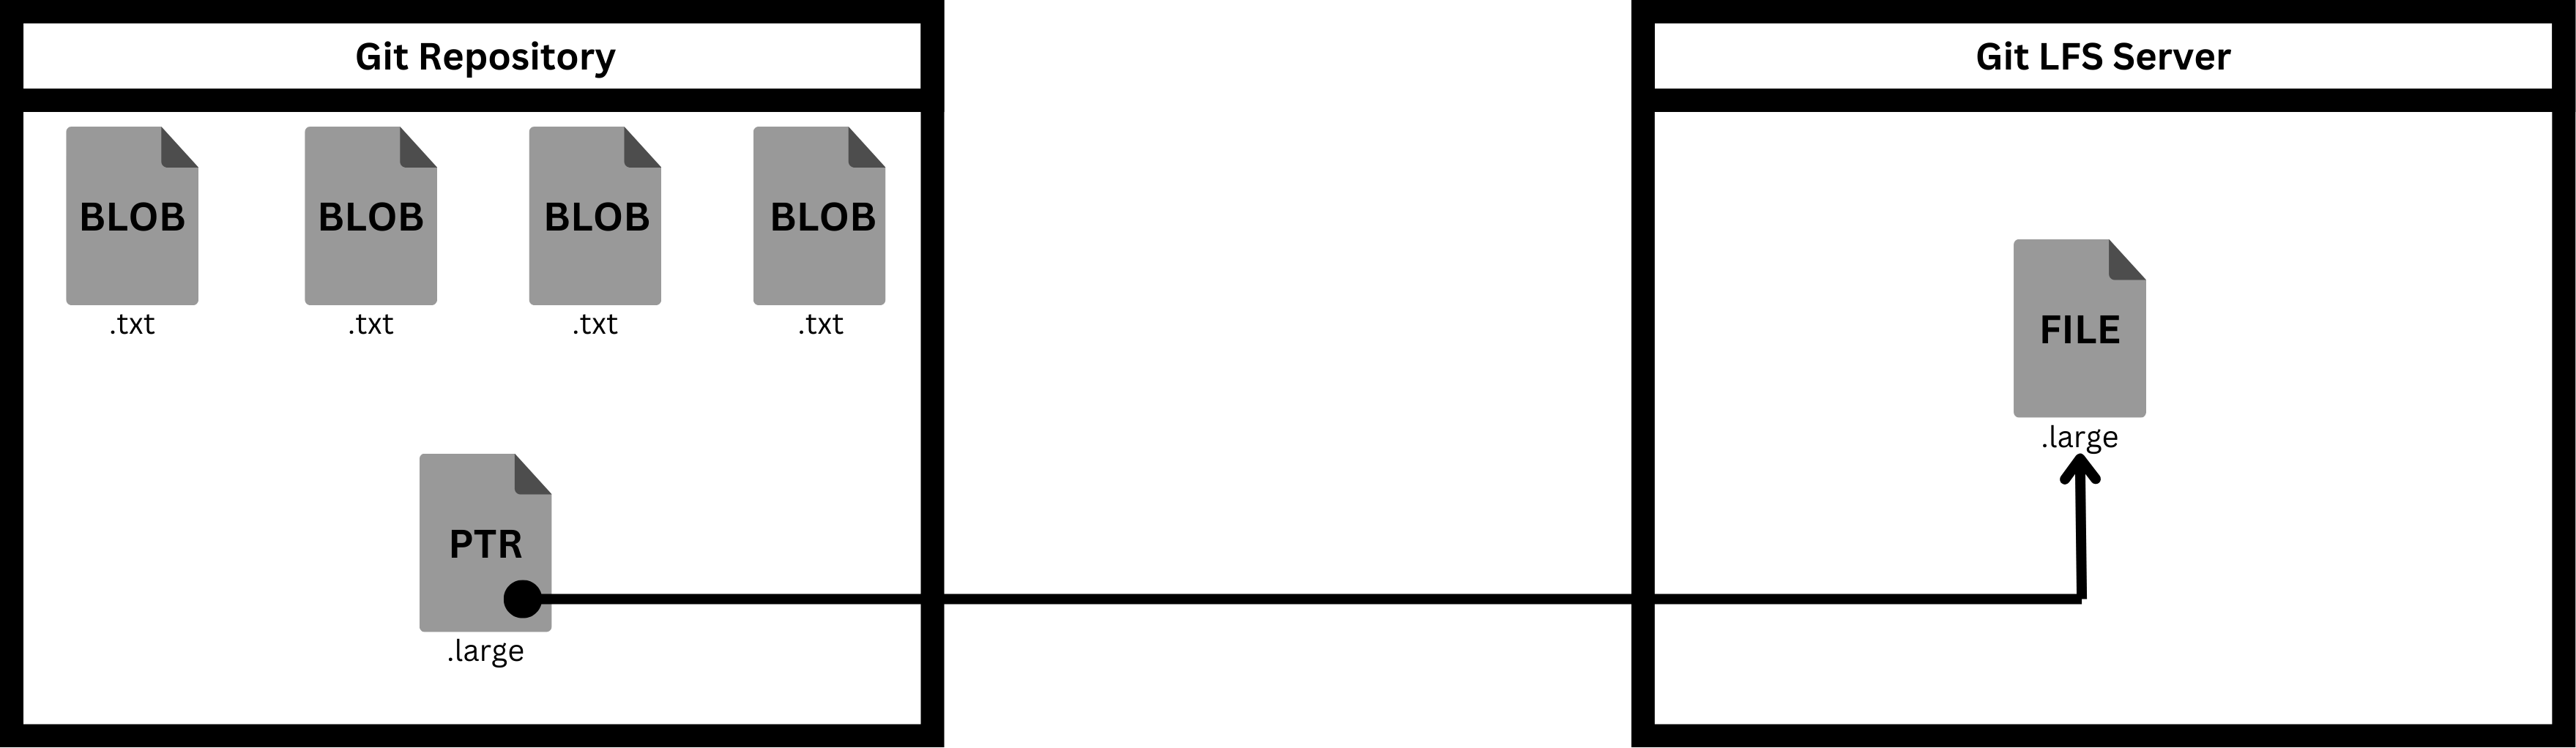
\includegraphics[width=0.8\linewidth]{figs/lfs-pointer.png}
    \caption{Explicative image that shows how LFS establishes a pointer to the remote LFS server.}
    \label{fig:LFSPointer}
\end{figure}

Whenever a branch containing the large file is checked out, its contents are downloaded from the LFS server. In case the contents of the file are modified, the new version of
the file is uploaded to the LFS server, which in turn generates a new version of the pointer file and makes a request to store it at the repository, all of it made in a 
transparent way for developers.

\begin{figure}[H]
    \centering
    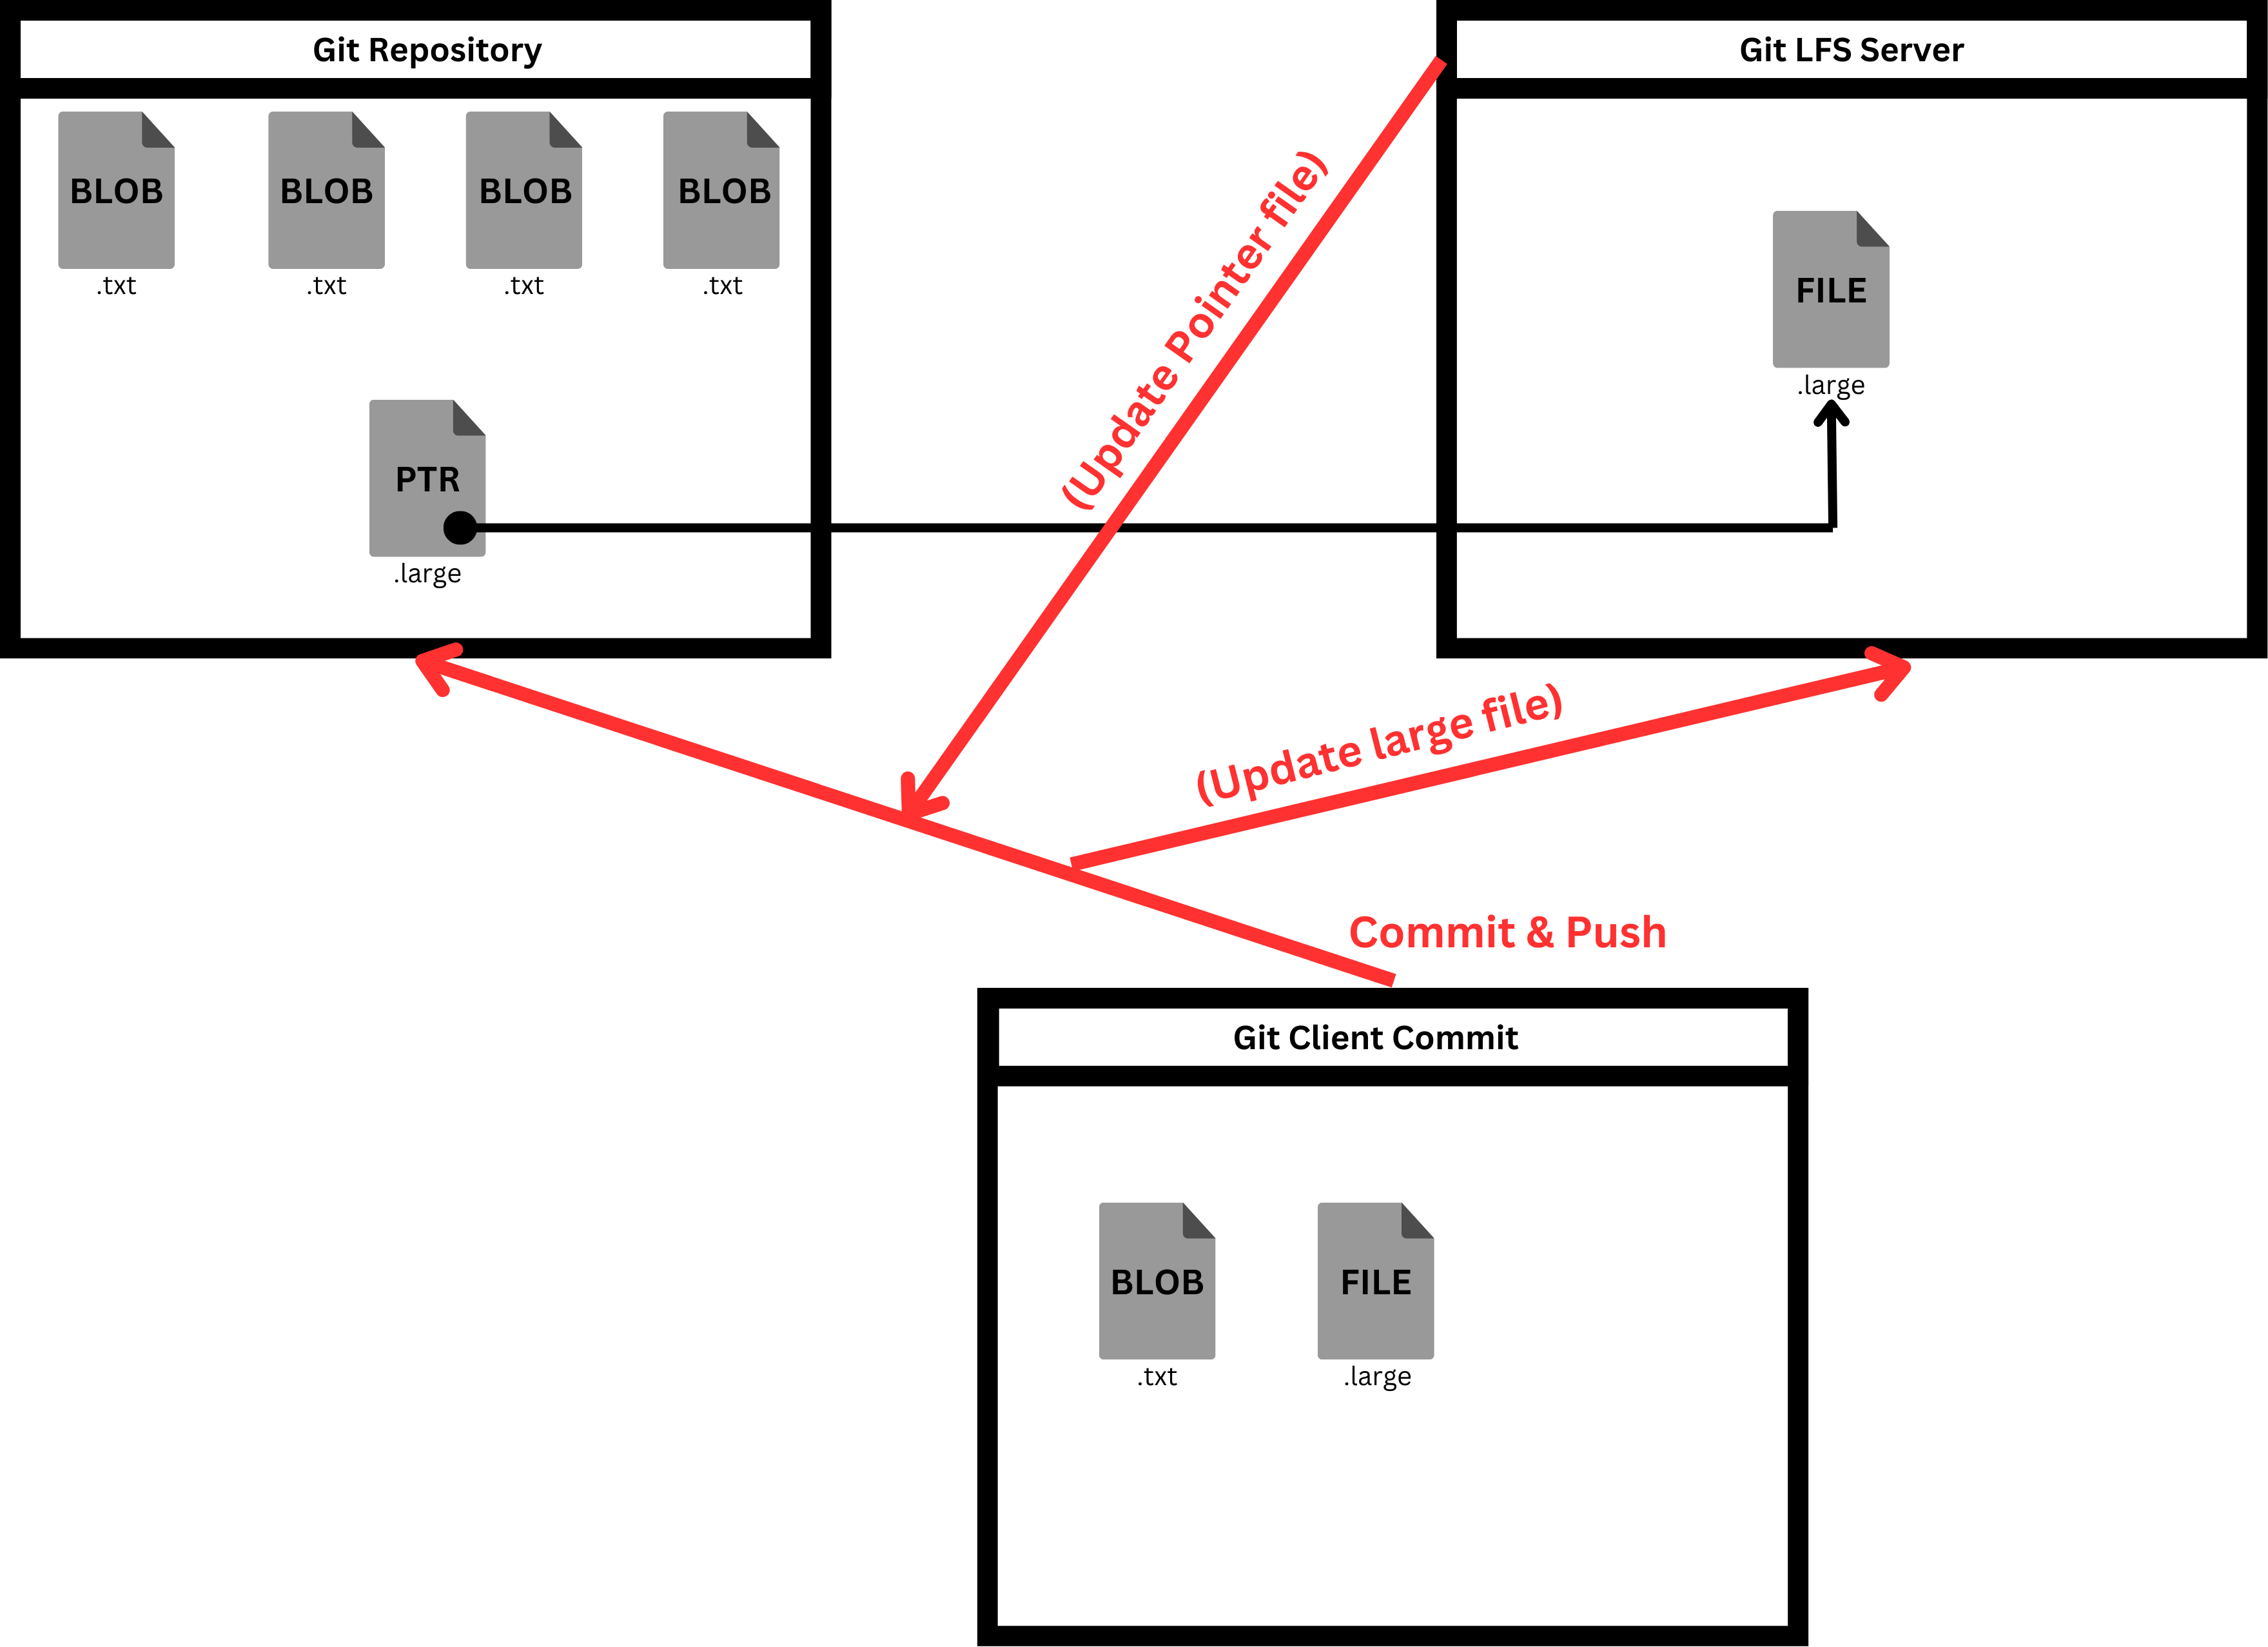
\includegraphics[width=0.8\linewidth]{figs/lfs-commit.png}
    \caption{Diagram of the process LFS performs to carry out the commit operation over a registered large file.}
    \label{fig:LFSCommit}
\end{figure}

With this simple mechanism, it is possible to transparently version and store large files in a Git repository without causing a huge overhead when performing operations at 
the Git repository.

\newpage
\subsubsection{Advantages and disadvantages of Git LFS}

\paragraph{Advantages of Git LFS}

\begin{itemize}

    \item \textbf{High Performance}: The mechanism for storing large files (a few gigabytes large) in Git enables the management of these kind of files as well as not letting
    their size slow down the transactions or using too much memory.

    \item \textbf{Ease of use and familiarity: }The Git LFS command line interface is simple and easy to use for users already familiar with Git, given the similarity between 
    the commands of both interfaces. This considerably flattens the learning curve of the tool.
\end{itemize}

\paragraph{Disadvantages of Git LFS}

\begin{itemize}

    \item \textbf{Not scalable:} If Git LFS were to be used in a distributed environment, it would not scalable due to the fact that it needs to be installed on every end user's
    system, and configured for every repository.

    \item \textbf{Limited in storage:} Git LFS has limited remote storage capacity (2 GB per file), falling thus too short on storage capacity for a project like MADTrack, which
    aims to handle datasets whose weight is counted in hundreds of gigabytes

    \item \textbf{Performance loss for very large files:} According to a Git LFS blog in Assembla \cite{assemblagitlfs}, some performance losses were reported upon storing 
    multiple very large files in a single Git LFS server. This serves as proof that Git LFS has difficulty in managing files heaver than a few gigabytes.

    \item \textbf{Difficult integration:} For integrating Git LFS into a system, it is also required to have Git Credential Manager installed (as a dependency).
    This dependence makes it a less modular solution than other possible alternatives.

\end{itemize}

\subsection{Data Version Control (DVC)}

Data Version Control (DVC) is an open-source, data-science-specialized software tool that provides mechanisms for easy data and experiment management, as well as 
for Machine Learning pipeline automation. It can be used in the form of an \acrfull{IDE} extension, a command line interface, or even as a library of the Python
programming language. It is designed for aiding data science and machine learning teams.

\subsubsection{How does DVC work?}

According to its official documentation \cite{dvcdocs}, the design of DVC is based on three main principles: codification (being able to define any important aspect
of a Machine Learning project by making use of a metafiles, making room for best practices and engineering toolsets), versioning (it uses the Git workflow to enable 
teams to collaborate and share their work), and secure collaboration (enabling selective collaboration and access to all aspects of a project).

DVC has a very similar feel and workflow as Git, thanks to its operation on top of it. The storage space problem is solved by means of special files: DVC metafiles. 
This files have the dvc extension and serve as placeholders to track data files and directories. Additionally, there are other types of files, like the ones with the 
\texttt{dvc.yaml} extension, which have the purpose of modeling entire Machine Learning projects, or \texttt{.dvcignore} files, which are used to ignore certain files or 
directories. The files in DVC are stored in certain local or remote storage systems, but DVC treats them all under the name of DVC remote.

DVC handles repositories as DVC projects, which are initialized by the use of \texttt{dvc init}. Once a project is initialized, DVC offers a wide-ranging variety Of
mechanisms to handle the configuration of the files and directories from a dataset. The \texttt{dvc add} command must be used for tracking an item.

Upon adding an item into DVC's tracking system, both a placeholder named \texttt{<filename>.dvc} will be created, as well as a \texttt{.dvcignore} file (if not
existing yet) within the target's directory. The former will store the changes on the file or directory, whilst the other will prevent the original file or directory from
being tracked by Git.

Furthermore, DVC is also able to retrieve or push data from or to a specific DVC remote using the \texttt{dvc pull/push} command, and to load a previous version of a tracked 
item after a checkout on the Git repository has been made, by making use of \texttt{dvc checkout}.

\subsubsection{Advantages and disadvantages of DVC}

\paragraph{Advantages:\cite{dvcoverview}}

\begin{itemize}
    \item \textbf{Specialisation: } DVC differs from other more general toolsets by its specialisation in the niche opened by emerging ML frameworks. DVC is aims to be used 
    by Machine Learning teams for Artificial Intelligence and Data Science projects. Hence, the options provided by the tool easily adjust to the needs of these specialists.

    \item \textbf{Easy to learn: } DVC working on top of Git repositories and taking inspiration of their workflow makes it very easy to learn and understand. Most of DVC's 
    commands are alike to those of Git.

    \item \textbf{High performance: } DVC has been designed to easily manage files the size of an actual neural networks dataset or a machine learning model. Hence, it makes
    it very efficient for these specific cases.

    \item \textbf{Compatibility: } DVC's remotes can be either local directories or remote storage systems. This may facilitate integration with the existing storage providers
    of the company.

\end{itemize}

\paragraph{Disadvantages:\cite{dvcoverview}}

\begin{itemize}
    \item \textbf{Slightly inflexible: } DVC will not accept an organisationally undefined environment in terms of architecture or design of the Machine Learning workflow. Teams must have a 
    well-defined pipeline and metrics of the model in order to take full advantage of DVC's modeling tool.

    \item \textbf{Workflow imposition: } DVC requires a Git workflow. This makes it very difficult to use the tool in projects where this workflow is not well-suited.

\end{itemize}

\subsection{MLFlow}\label{sec:mlflow}

MLFlow is an open-source project, specifically built with the objective of providing assistance in the Machine and Deep Learning process, managing the full lifecycle of 
projects of this nature and ensuring its traceability and reproducibility\cite{mlflowdocs}.

MLFlow offers mechanisms for Machine Learning model tracking and registry (handles configuration management), evaluation (it is able to track and compare different 
versions of a model) and reciping (provides guiding for structuring a Machine Learning or Deep Learning project).

This tool has gained particular popularity, since it is being used by the great companies, such as Microsoft, META and TOYOTA.

\subsubsection{How does MLFlow work?}

MLflow has a complex workflow consisting of various components, which are thoroughly explained in the following paragraphs \cite{mlflowtracking}.

The MLFLow tracking \acrfull{API} is present in many programming languages (Python, R, Java and REST) and is part of the many components of MLflow, having the aim of 
providing the sufficient logging mechanisms for tracking a \acrshort{ML} or \acrshort{DL} project, including logging of parameters, code versions, metrics and output files.

In figure \ref{fig:MLFlowScenarios}, an overview of the most common MLFlow deployment architectures show the different possibilities MLFlow can be used:

\begin{figure}[H]
    \centering
    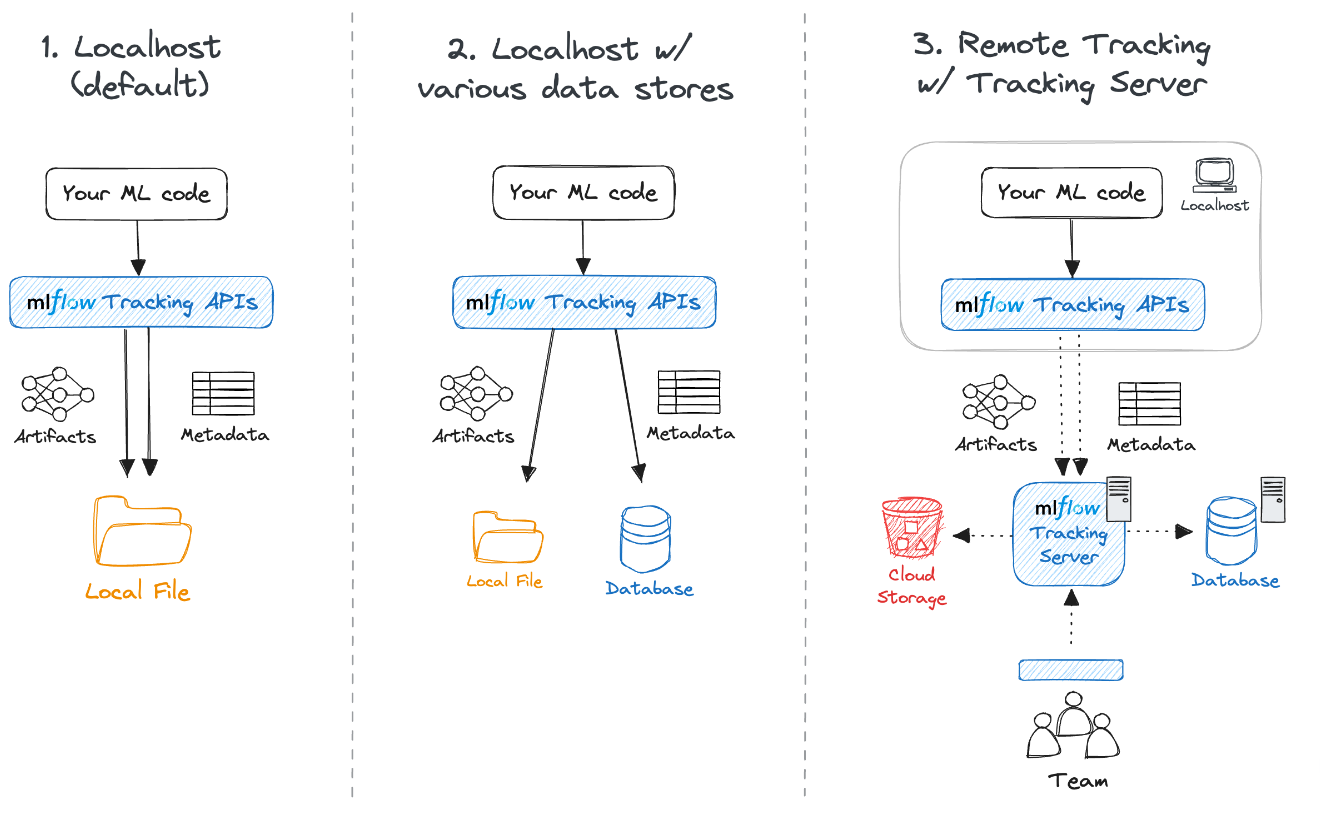
\includegraphics[width=0.8\linewidth]{figs/mlflow-tracking.png}
    \caption{Diagram showing the different use scenarios of MLFlow. Source:\cite{mlflowtracking}}
    \label{fig:MLFlowScenarios}
\end{figure}

In total, three use scenarios can be identified:

\begin{itemize}
    \item \textbf{Localhost scenario: } MLflow stores and logs ML model metadata and artifacts inside a local file system directory.
    
    \item \textbf{Localhost with data stores: } Similar to the previous setup, but it also stores and logs data files in a remote file
    system or database.

    \item \textbf{Use of a remote tracking server:} The ML code is tracked by the API into a remote HTTP tracking server, which stores 
    it in a remote storage and allows storing and retrieving items without directly accessing the storage media.

\end{itemize}

Apart from the API, there are more relevant components, such as the model registry. MLFlow's model registry provides the MLflow toolset 
with mechanisms for model lineage, versioning, aliasing, tagging and annotation. This component of MLflow can be accessed by running a 
proper MLflow server and using a backend storage medium. Whenever a model is desired to be registered, it is needed to be logged first.
Some basic concepts to understand how this registry component works are:

\begin{itemize}
    \item \textbf{Registrable model: }a model created from an experiment or run and logged with one of the model methods. Currently, MLFLow supports SKLearn, Pytorch and
    TensorFlow models.

    \item \textbf{Registered model: }a model registered with using the model registry. It contains a unique name, versions, aliases, tags and metadata.
    
    \item \textbf{Model version: }representation of a stage in the evolution of a model. Any newly registered model is assigned version 1.
    
    \item \textbf{Tag: }quality or set of qualities expressed about a model, expressed as a key-value pair. Allows model categorization.
    
    \item \textbf{Alias: }is a mutable, named reference assigned to a model version.
    
    \item \textbf{Annotation: }Markdown styled comment on a model in any model version. It used for describing and expressing relevant 
    information to the project's collaborators.
\end{itemize}

MLFlow also provides its users with a friendly \acrfull{UI} that is available on the cloud, and accessible by means of an internet browser. Before coming in detail
about the provided functionalities, some concepts may be introduced first:

\begin{itemize}
    \item \textbf{Model run: }process that englobes the training, validation and testing of a model.
    \item \textbf{Experiment: }representation of a set of model runs that share a common purpose, e.g. An experiment for ship segmentation models.
    \item \textbf{Artifact: }a file whose content is relevant to a certain model run.
\end{itemize}

This interface allows the navigation through the different registered experiments using a stack panel, as well as a comparative stack view of the different model runs, 
along with the parameters, metrics and datasets obtained within each run, which can be sorted according to the users' needs. The interface also provides menus for 
visualizing the different models and artifacts within a model run.


\begin{figure}[H]
    \centering
    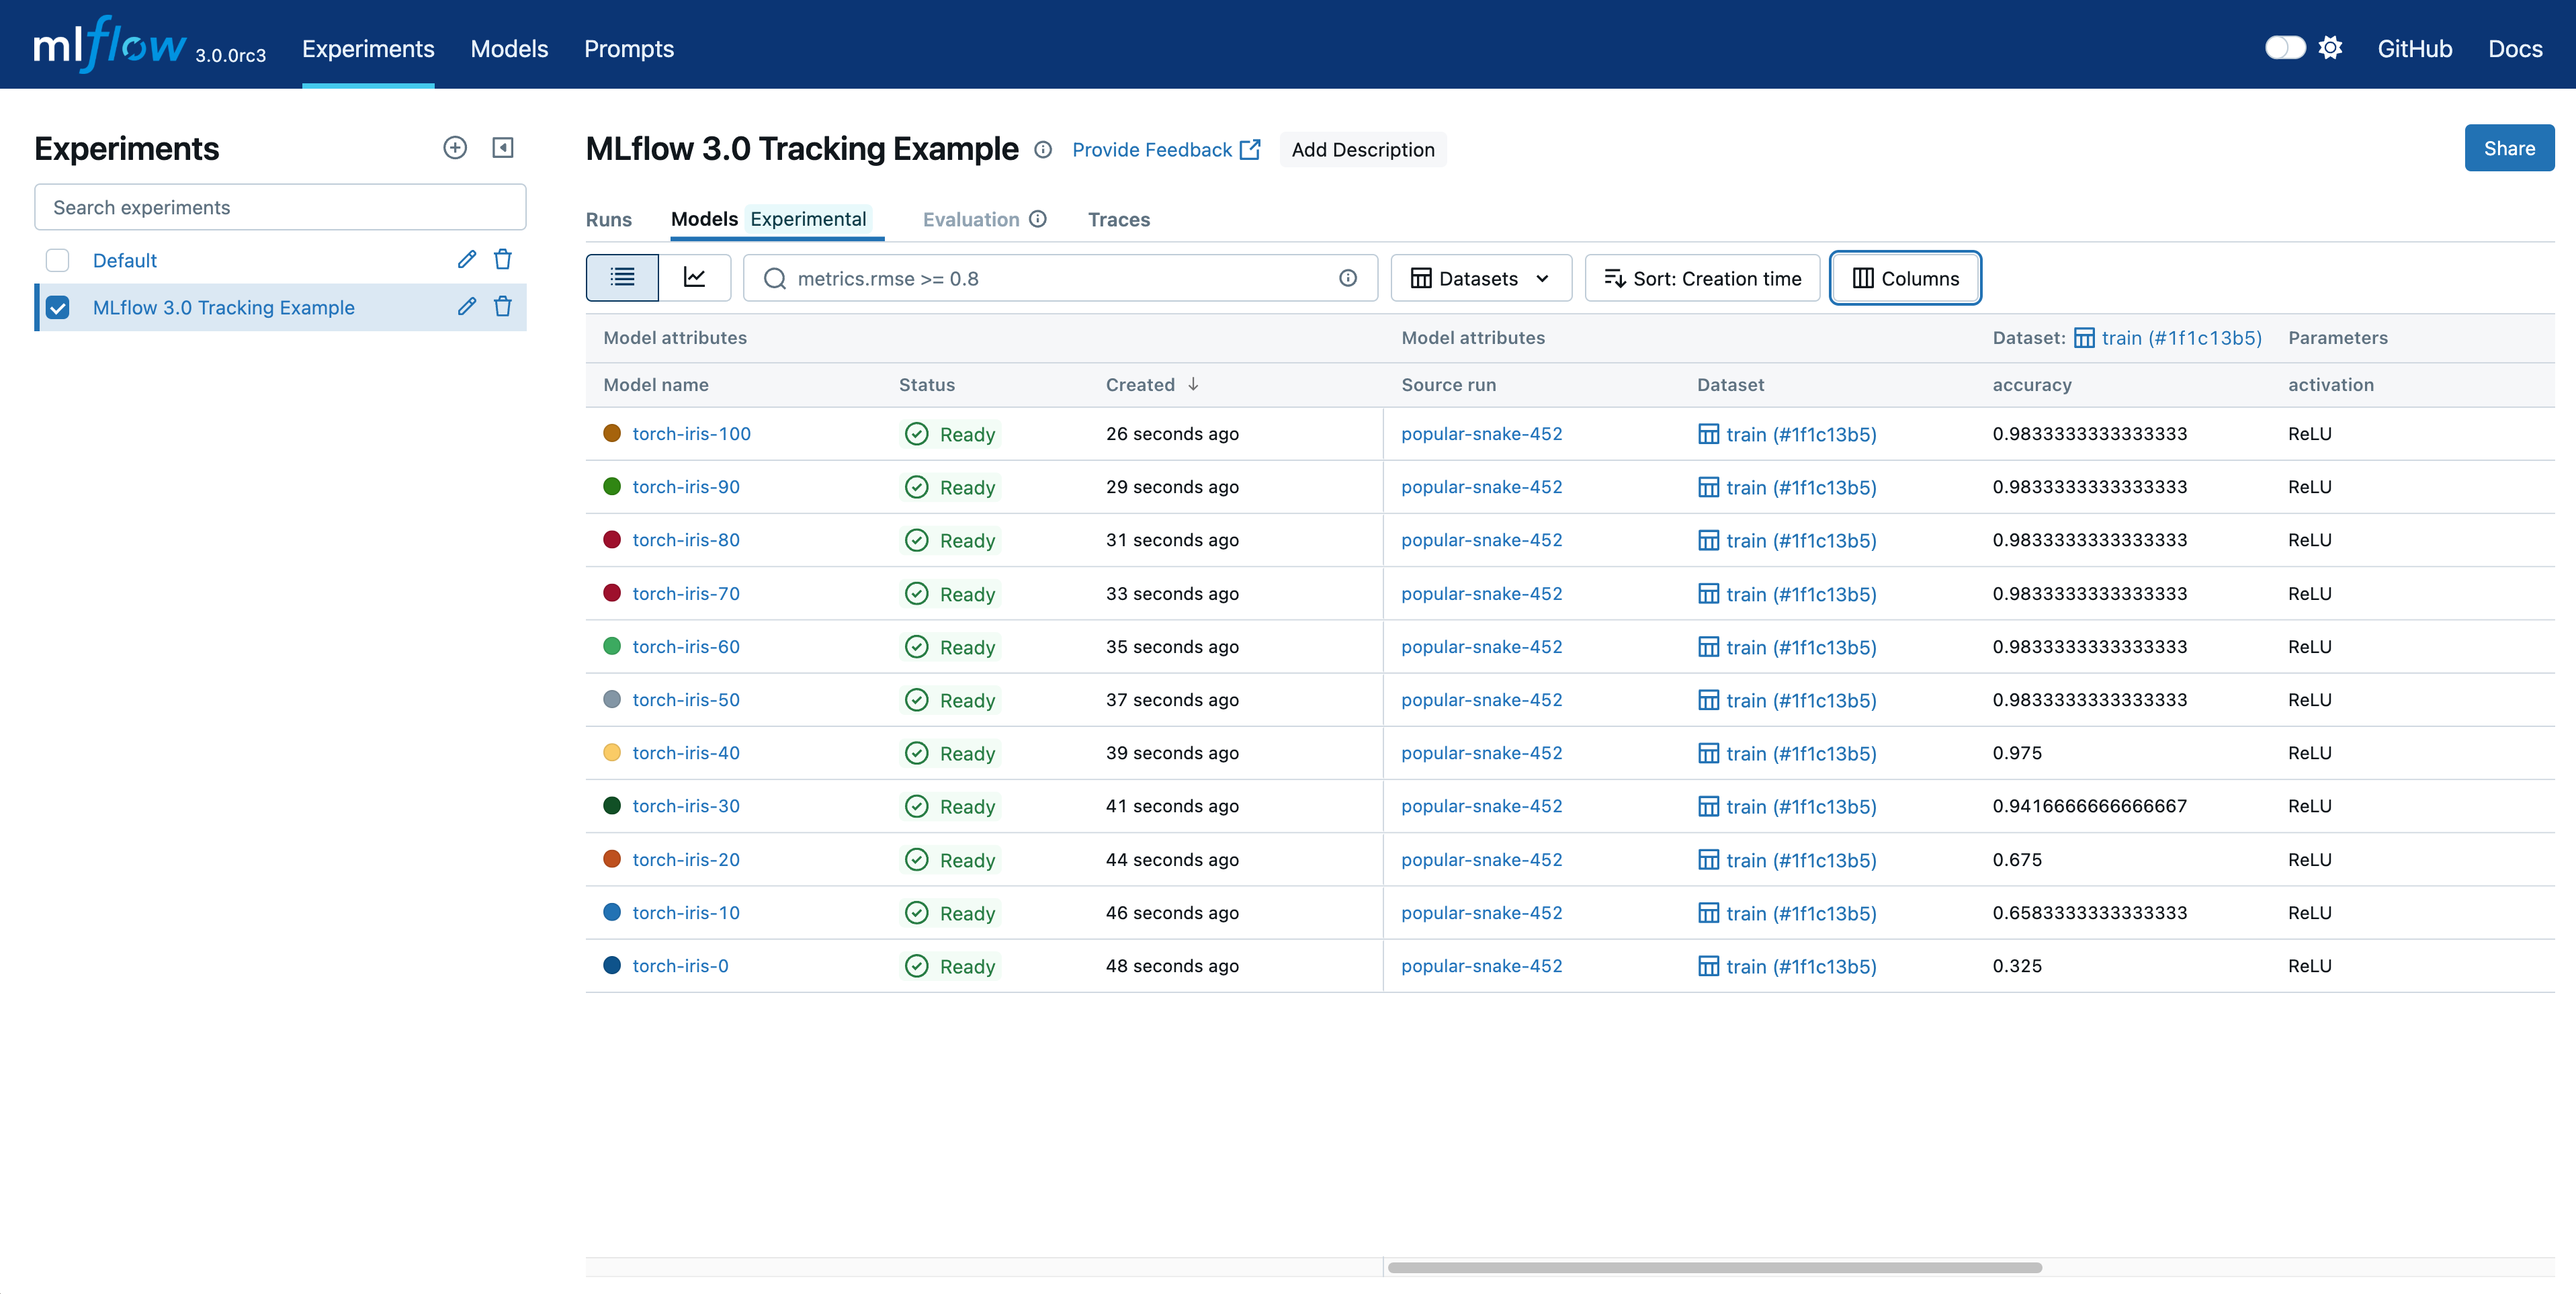
\includegraphics[width=0.8\linewidth]{figs/mlflow-ui.png}
    \caption{MLFLow's \acrshort{UI} showing the list of runs contained within an experiment. Source:\cite{mlflowtracking}}
    \label{fig:MLFlowUI}
\end{figure}

\subsubsection{Advantages and Disadvantages of MLFlow\cite{mlflowproscons} }

\paragraph{Advantages:}

\begin{itemize}
    \item \textbf{Complete: }this tool excels at managing \acrshort{ML} and \acrshort{DL} models, with all the complexity it takes for tracking 
    their evolution, versioning and even comparing them with other models.

    \item \textbf{Easy to learn: }apart from all the complexity hidden for managing the components of the tool, MLflow has an easy installation method
    and an intuitive \acrshort{UI}. The documentation provides users with a wide-ranging set of quick tutorials that will help them get started in the
    minimum amount of time.

    \item \textbf{Flexibility: }in the documentation, it is possible to see many tutorials which import libraries libraries related to the Machine Learning 
    toolset with MLflow libraries, showing its versatility and integrability with many other toolsets related to Artificial Intelligence development. 
    A quite desireable quality for a tool with this role inside a \acrshort{ML} project.
\end{itemize}

\paragraph{Disadvantages:}

\begin{itemize}
    \item \textbf{Insufficiency in dataset management: }MLflow may be a great tool for managing the whole lifecycle of projects and \acrshort{AI} models, 
    but it lacks of mechanisms this good for dataset configuration management. This means that either way, another tool that manages specifically the datasets' lifecycle
    is needed, leading to integration, which leads in turn to higher complexity.

    \item \textbf{Difficult to dominate: }MLflow provides its users with many tutorials to give them a sense of how this tool works in record time. Nevertheless,
    the fact that the tool has a steep learning curve is undeniable. Its varied set of components makes it a complex tool with many possibilities, and it is difficult
    to gather the knowledge to master them all.
\end{itemize}

\subsection{Neptune.ai}

Neptune.ai is a \acrshort{PaaS} that allows users to easily supervise and monitor \acrshort{AI}/\acrshort{ML} foundation model trainings and lifecycle. This set of 
functionalities classify under the definition of an \textbf{experiment tracker} application category. The features offered by Neptune include a combination between
a database and and a dashboard, with logging support for machine learning models for Python, mostly like MLflow does, but adding the incorporation of a decent system
for dataset versioning.

\subsubsection{How does Neptune.ai work?\cite{neptunedocs}}

Neptune.ai's system consists of two main components:

\begin{enumerate}
    \item \textbf{Neptune.ai's Python library: }an \acrshort{API} that can be found inside a Python library, used for logging and querying metadata extracted from model
    building. The tool also offers a \acrfull{CRUD} interface for users and workspaces, as well as various monitoring mechanisms.

    \item \textbf{Neptune.ai's web application: }a web application that enables users to visualize, compare, monitor and collaborate in \acrshort{AI} projects.
\end{enumerate}

The interactions between different clients and servers can be described within figure \ref{fig:NeptuneDiag}. As shown, various clients that have Neptune's library installed make request to an
active Neptune Server, where the web application is also deployed in. The interaction between the users and the web application is regulated by the use of the Python library, creating a workspace
for every existing organization, and a project per Machine Learning task.

\begin{figure}[H]
    \centering
    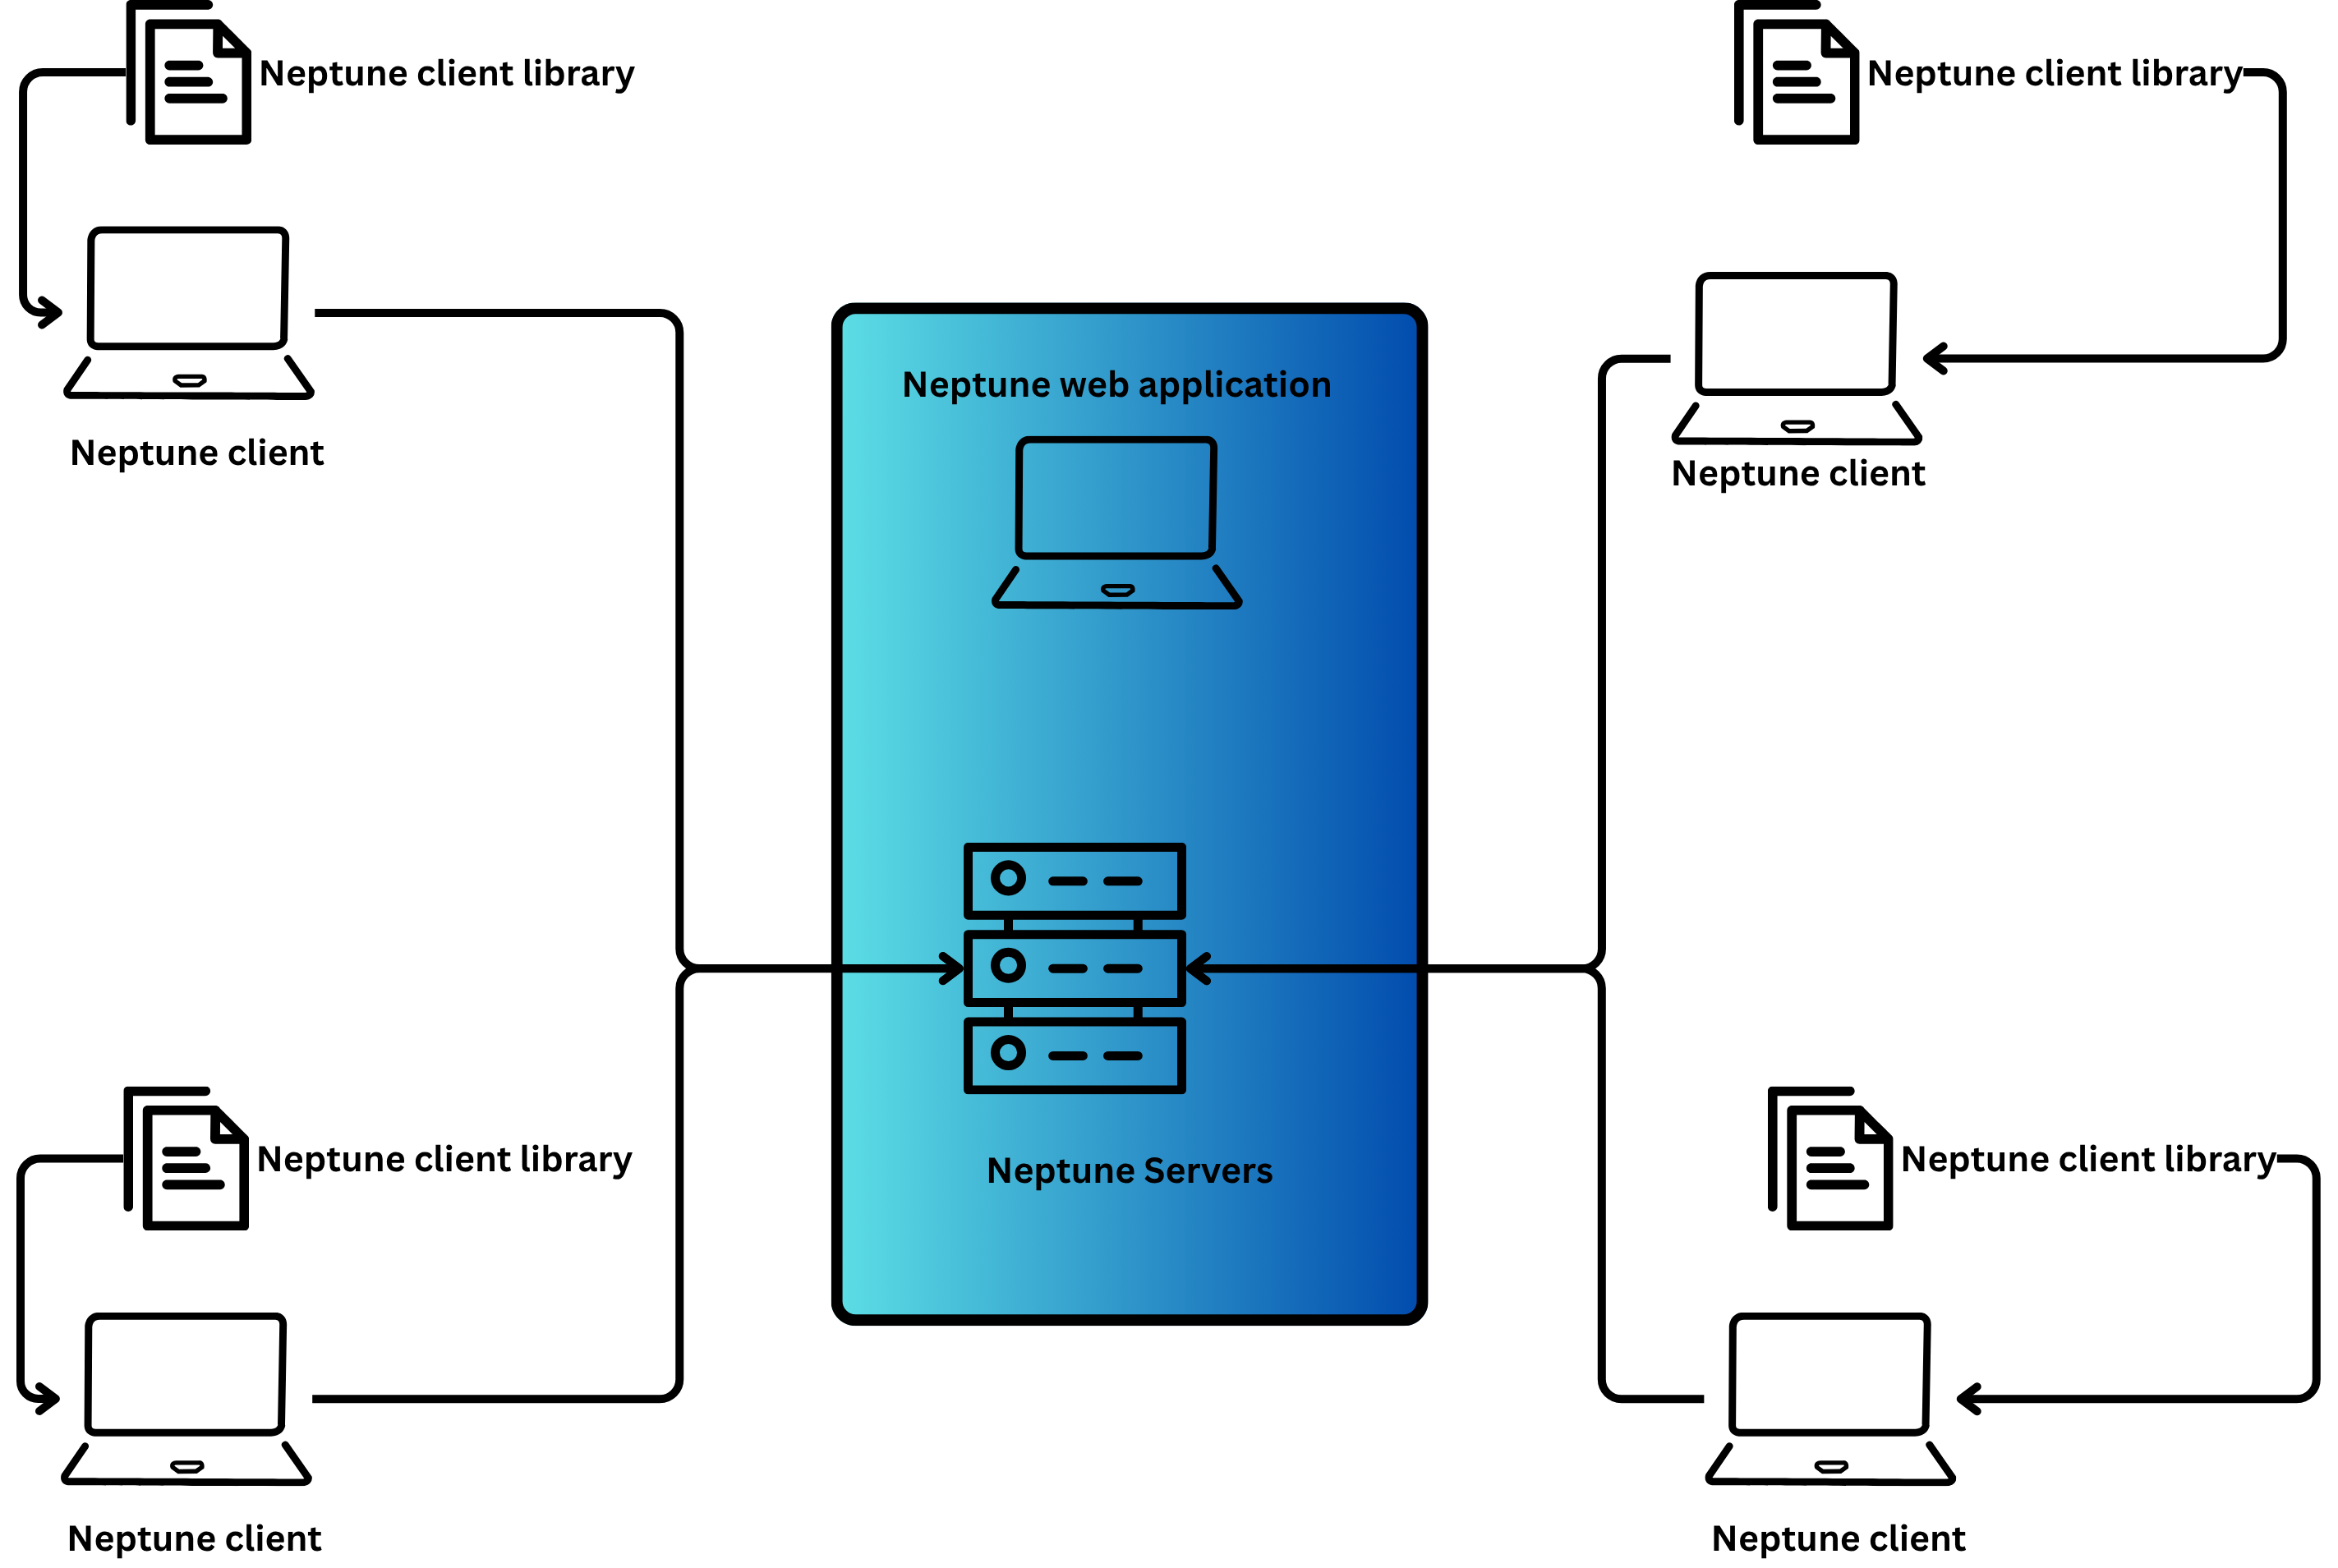
\includegraphics[width=0.8\linewidth]{figs/neptune-clientserver.png}
    \caption{Interaction between Neptune clients and a Neptune server.}
    \label{fig:NeptuneDiag}
\end{figure}

In order to better understand Neptune's environment, some concepts shall be introduced:

\begin{itemize}
    \item \textbf{workspace: }a space for projects and team members with a specific storage amount, created with or without permission for public projects, and with one 
    or more (non-human) service accounts. The storage limits of a workspace can be changed by the workspace administrators, but it may come with a fee charge (The free
    plan of Neptune only provides 200GB storage).

    \item \textbf{Service accounts: }privileged Neptune accounts that do not belong to human entities, and have the purpose of automating tasks that are normally performed
    through a human account. These accounts are workspace-specific and controlled by administrators.

    \item \textbf{Project: }represents the concept of a Machine Learning task. It registers all the tracked runs and shows them to all authorized members, allowing exploration and 
    analysis. Projects have three visibility levels: Workspace (grants access for any of the project's workspace members), Public (available to anyone in the Internet)
    or Private (available only to the chosen members).

    \item \textbf{Run: }a tracked experiment of a project. It contains model-building metadata. They are created every time a model is trained or retrained and
    each time a model performs an inference by means of a executable script.

    \item \textbf{Model: } represents an \acrshort{AI} Model. Is a collection of metadata common to all the model versions of the same model.

    \item \textbf{Model Version: } represents the version of a Machine Learning model. It consists of metadata common to a single version of a model.

\end{itemize}

Neptune also integrates with most of the Machine Learning toolsets available in the market. Making it feasible for integration in the project concerning this Final
Degree Project. It counts with logging callbacks in order to easily integrate it around any model fitting.

Finally, Neptune.ai only takes a little knowledge of environment variables and terminal commands in order to run its \acrshort{UI}, from which all the logging and
metrics can be consulted and the metadata and performance can be easily visualized.

Once the main components of Neptune have been introduced, a generic workflow would have the following steps:

\begin{enumerate}
    \item Add some lines of code before training a model. Just the ones for importing the right libraries and setting the logging callbacks.
    \item Use the Neptune.ai web application to browsed the logged metadata during the training.
    \item Visualize and compare run metadata.
\end{enumerate}

\subsubsection{Advantages and disadvantages of Neptune.ai\cite{neptuneproscons}}

\paragraph{Advantages:}

\begin{itemize}
    \item \textbf{Scoped for project needs: }Neptune.ai manages both models and dataset versioning, so no additional integrations are needed.
    
    \item \textbf{Designed for collaboration: }Neptune.ai is designed to be used in a collaborative environment, so it easily tracks the progress of a project made by 
    any team member.

    \item \textbf{Standardized: }this tool complies with SOC2\cite{SOC2}, a standard for security and compliance.
    
    \item \textbf{Ease of use: }Neptune.ai is a Python API package that can be easily installed and used in any Python project. It also allows the easy visualization the
    metadata of models and their training performance by using the web application.
\end{itemize}

\paragraph{Disadvantages:}

\begin{itemize}
    \item \textbf{Non-scalable: }the tool is not scalable to large datasets as the storage is limited, at least, in the free plan.
    \item \textbf{Limited by language: }The tool only provides a single Python package, which is incompatible with other languages.
\end{itemize}

\subsection{Comet.ml}

Comet.ml is another \acrshort{PaaS} oriented to \acrshort{AI} model evaluation, experiment tracking, and production monitoring, with particular expertise in \acrfull{LLMs}.
It is used by companies like UBER and NETFLIX. It also provides a meeting point for all the \acrshort{ML} development platforms (and even those not aimed
exactly at developing this kind of models) and cloud infrastructure supported by providers like Amazon Web Services, Google Cloud and Azure.

\subsubsection{How does Comet.ml work?\cite{cometmldocs}}

Comet.ml is available as a Python package, a command line extension, and also provides an \acrshort{UI} for visualizing and managing information on experiments.

With the python package,Comet enables logging for three types of information: AI model metadata (key-value pairs, metrics, parameters, information about the system, 
and so on), Assets and data (unversioned files like images, models, confusion matrices), and artifacts (versioned assets, like datasets). Comet.ml will track all relevant
loggable assets until the code execution is over.

The user interface provides an option for customizing dashboard views, as well as for viewing and comparing experiments. It well combines with popular libraries like 
Scikit-Learn, Optuna and the self comet optimizer, helping users to find the optimal set of hyperparameters for their models. Comet also offers a model registry to 
track and version models.

Comet also introduces some concepts such as organization, workspace, project and \acrfull{MPM}. Most of these being equivalent to the definitions provided in earlier
subsections.

\subsubsection{Advantages and Disadvantages of Comet.ml\cite{cometmlproscons}}

\paragraph{Advantages: }

\begin{itemize}
    \item \textbf{Ease of integration: }Comet is easy to integrate with other services and platforms, like Python Flask.
    \item \textbf{User-friendly interface: }Comet has been recommended by some G2 members as a tool with a very intuitive user interface.
    \item \textbf{Suited for collaboration: }Comet is designed for collaborative environments, where multiple members work at a time.
\end{itemize}

\paragraph{Disadvantages: }

\begin{itemize}
    \item \textbf{Costly: }The free plan of Comet.ml is very limited, while the premium plans scale up from 50 dollars a month.
    \item \textbf{Limited Customization: }Comet.ml does not provide as much customization options as other tools, which may be disappointing for the price of the 
    service.
    \item \textbf{Limited by language: }The exclusive availability of the tool in the Python programming language restricts its flexibility.
\end{itemize}

\subsection{Weights and Biases (WandB)}

Weights and Biases, also known as \emph{WandB}, is a \acrshort{PaaS} dedicated to provide data scientists and AI developers with a toolkit that facilitates the production
process of Artificial Intelligence models. It provides support for experiment tracking, hyperparameter sweeping, model registry and workflow automation, among many 
others.

\subsubsection{How does WandB work?}

WandB makes use of a set of lightweight, interoperable tools for managing the configuration of AI models, as well as for storing, displaying and sharing results. This 
makes the platform highly suitable for teams. It is available as either as Python and Javascript libraries, a Command Line Interface (CLI) and an interface that 
functions with an interface specialized in data addition.

Like most platforms, The main workflow consists of adding some code from the libraries prior to carrying out the training process, which connect with the cloud platform,
for later tracking and visualization.

Some of the functionalities offered by WandB are:

\begin{itemize}
    \item \textbf{Experiment tracking: }it allows to track the progress of a project made by any team member.
    \item \textbf{Sweeping: }the platform itself lets developers visualize the impact of the hyperparameters on the performance of the model. The platform is also able to 
    perform open-source algorithms to infer the best possible values for the hyperparameters, visualizing all past and suggested configurations of the hyperparameters
    over a dashboard that the team can visualize.
    \item \textbf{Model Registry: }provides a way to govern over the trained models over their whole lifecycle.
    \item \textbf{Workflow trigger automation: }it offers tools for streamlining the learning pipeline and implementing sophisticated \acrfull{CICD} processes by means of 
    automatic workflow execution.
\end{itemize}

\subsubsection{Advantages and disadvantages of WandB}

\paragraph{Advantages: }

\begin{itemize}
    \item \textbf{Familiarity: }while gathering information to transform it into requirements, process detailed in coming chapters, it was revealed that some of the end users of this project already 
    using this tool.

    \item \textbf{Versatility: }WandB can handle most (if not every) of the steps of the Artificial Intelligence models' lifecycle.

    \item \textbf{User-friendly: }WandB was reported in an article from Netguru\cite{wandbprosandcons} as a tool with a very intuitive user interface.
    
    \item \textbf{Code efficient: }The platform itself requires little amounts of code to be able to carry out the complete WandB workflow.
    
    \item \textbf{Suited for embedded system integration: }WandB can generate reports on power consumption and efficiency over the training and inference processes of 
    an AI model, which can be very useful for embedded AI developers like the intended end users of the project.
\end{itemize}

\paragraph{Disadvantages: }

\begin{itemize}
    \item \textbf{Limited by language: }WandB is only available in Python and Javascript, and not in other languages.
    \item \textbf{Costly: }the free plan of WandB is very limited, while the premium plans scale up from 50\$/month.
\end{itemize}

\section{Adoption of AI and Dataset Configuration Management Technologies}

This page provides the resulting overview from the exploration of other areas or companies that have already adopted a machine learning and dataset versioning platform, 
if possible in a similar context the one intended for this Final Degree Project.

\subsection{Microsoft}
In \emph{section \ref{sec:mlflow}}, it was explained how MLFlow was used by various widely known companies, one of these being Microsoft. This company has indeed 
a section explaining how this tool works in their system and how they use it for integration with another tool: Ray\cite{microsoftmlflow}. Both of them are integrated 
as libraries in Python, and Ray tasks can be logged using the functions offered by MLfLow, thus proving the ease of integration that characterizes MLFlow.

\subsection{WIX}
The cloud website infrastructure and \acrshort{PaaS} provider WIX is a company that, similarly to Microsoft, has chosen to use MLFlow as part of the tools integrated in
the platform (as stated in \emph{section \ref{sec:mlflow}}). They were specially interested in the integration of MLflow and Apache Spark to produce their very own Machine
Learning platform, taking advantage of the model registry component. A deep study of how WIX uses this platform is described in a Medium story\cite{mediumwix}.

\subsection{Edge Impulse}
In 2019, the company Edge Impulse released the platform with the same name into the market. This platform provides a near-to-full range of tools to support Machine 
Learning Operations and Deep Learning pipelines adapted to TinyML, which are embedded systems specialized in or designed for running Machine Learning models. The 
platform provides a set of visual interfaces to make Machine Learning accessible to anyone. Some of its features, like the EON Tuner, also offer support for automated 
operations within the pipeline, thus assuring a more efficient and effective workflow. Up to now, the only limitation or important feature this platform lacks is the 
\acrshort{IoT} device manager and production monitor\cite{edgeimpulse}.

\begin{figure}[H]
    \centering
    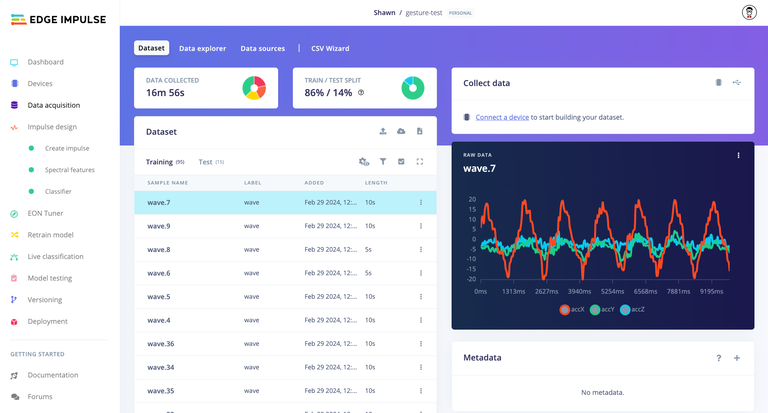
\includegraphics[width=0.8\linewidth]{figs/edgeimpulse-ui.png}
    \caption{A look at Edge Impulse's \acrshort{UI}. Source:\cite{edgeimpulsedocs}.}
    \label{fig:edgeImpulseUI}
\end{figure}


\include{./Caps/4_Desarrollo}
\include{./Caps/5_Conclusiones}

\singlespacing % Resto del documento siempre en espaciado sencillo
% -------------------------



% -------------------------
% --- BIBLIOGRAFÍA (Obligatoria)
% -------------------------
\bibliography{bibliografia} % Nombre del fichero .bib
\bibliographystyle{plain} % Elige el estilo adecuado.
% Estilos nativos incluidos con LaTeX (plain, abbrv, alpha, unsrt).
%
% plain: citación en estilo numérico. En la bibliografía las entradas
%        aparecen en orden alfabético.
%
% abbrv: Cita numérica. En la bibliografía los nombres aparecen
%        sólo con la inicial.
%
% unsrt: Cita numérica. La bibliografía por orden de cita en el texto.
%
% -------------------------
%        Estilos incluidos con BibTeX no nativos, pero populares
%        en ingeniería (no requieren paquetes adicionales).
%
% acm:   Cita numérica. En la bibliografía con los nombre de autores 
%        en mayúsculas y con ordenación alfabética.
%
% ieeetr:IEEE Transactions, con citación numérica y ordenación por orden 
%        de cita.
% -------------------------
% (FIN BIBLIOGRAFÍA)
% -------------------------


% -------------------------
% ANEXOS (si no los necesitas los puedes borrar o comentar)
% -------------------------
\appendix
\chapter{Annex: Big Figures}
\label{cap:AnexoA}

\begin{sidewaysfigure}
    \centering
    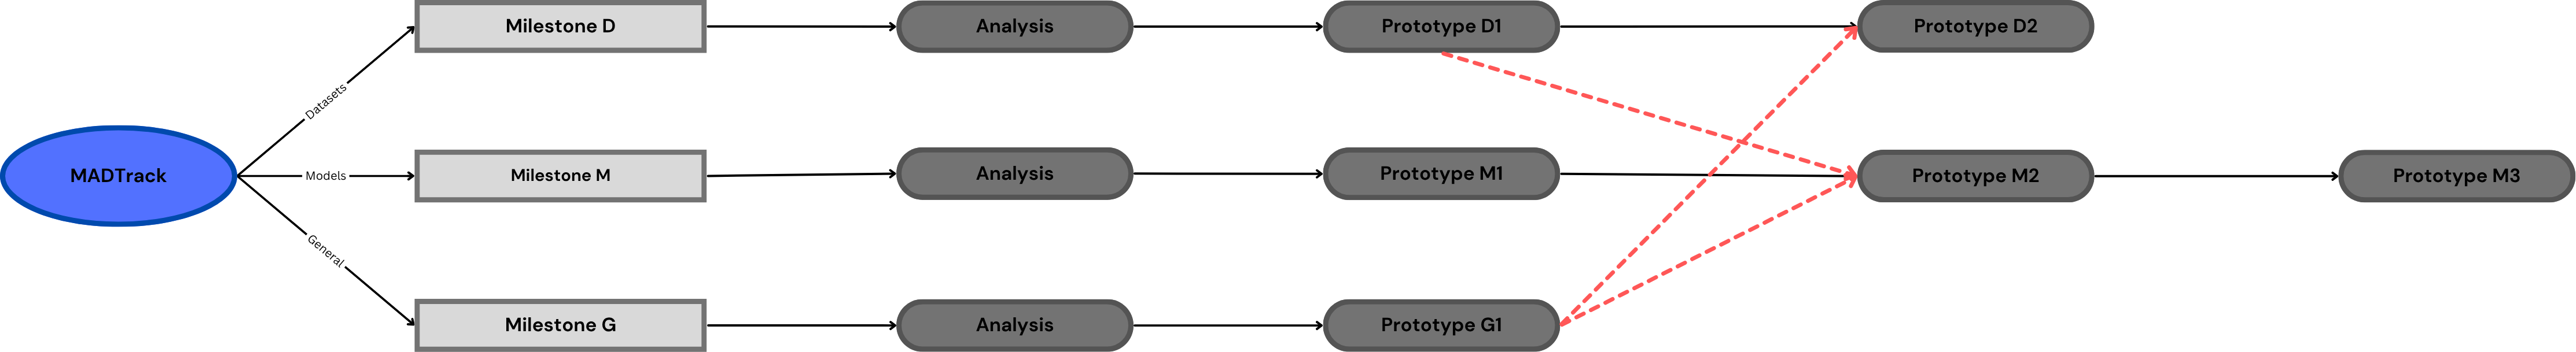
\includegraphics[width=\linewidth]{figs/MADTrack-roadmap.png}
    \caption{Iteration roadmap of the MADTrack project.}
    \label{fig:roadmap}
\end{sidewaysfigure}

\begin{sidewaysfigure}
    \centering
    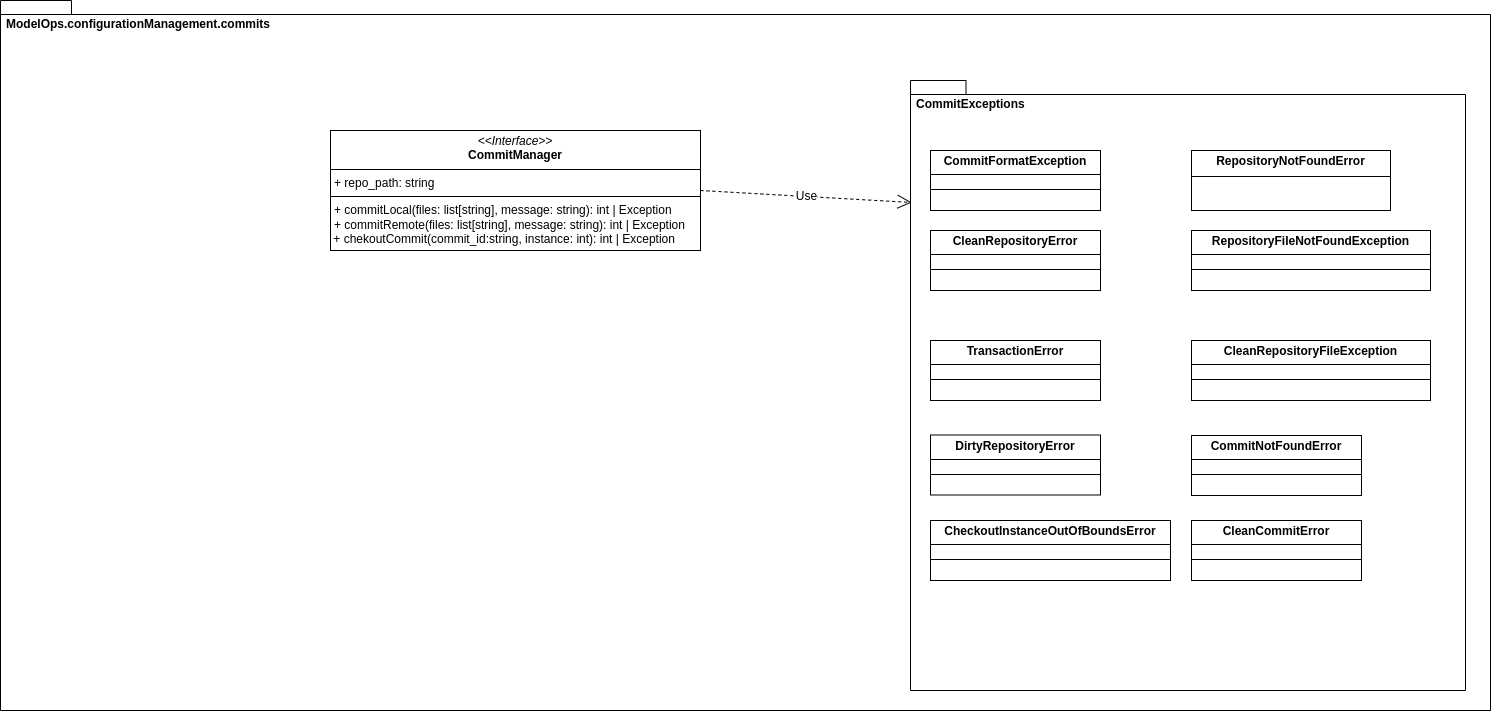
\includegraphics[width=\linewidth]{figs/G1-classDiagram.png}
    \caption{Class diagram for prototype \emph{G1}.}
    \label{fig:G1classDiagram}
\end{sidewaysfigure}
 % Apéndice A (opcionales)
\include{./Anexos/AnexoB} % Apéndice A (opcionales)
%--- (FIN DOCUMENTO)
\end{document}